
% This LaTeX was auto-generated from MATLAB code.
% To make changes, update the MATLAB code and republish this document.

\documentclass{article}
\usepackage{graphicx}
\usepackage{color}

\sloppy
\definecolor{lightgray}{gray}{0.5}
\setlength{\parindent}{0pt}

\begin{document}

    
    
\subsection*{Contents}

\begin{itemize}
\setlength{\itemsep}{-1ex}
   \item Exercise 1
   \begin{itemize}
       \item a
       \item b
       \item c
       \item d
       \item e
   \end{itemize}
\end{itemize}
\begin{verbatim}
clc
\end{verbatim}


\subsection*{Exercise 1}



\subsubsection*{a}

\begin{par}
Basic matrix and vector mathematics
\end{par} \vspace{1em}
\begin{verbatim}
fprintf("\n\nSolutions:\n\n");

fprintf("a)\n\n");

a = [2; 0; 5];
b = [4; 2; 1];
c = [0; 1; 0];

A = [2 5 2;...
    4 34 8;...
    4 5 2];

B = [2 4 0;...
    3 2 0;...
    6 2 0];


fprintf("a * bT = \n")
disp(a * transpose(b))
fprintf("a + b = \n")
disp(a + b)
fprintf("A * b = \n")
disp(A * b)
fprintf("AT * c = \n")
disp(transpose(A) * c)
fprintf("|A| = \n")
disp(abs(A))
fprintf("|B| = \n")
disp(abs(B))
fprintf("Ae-1 = \n")
disp(inv(A))
fprintf("Be-1 = \n")
disp(inv(B))
\end{verbatim}


\subsubsection*{b}

\begin{par}
Exercises from the mathematics course
\end{par} \vspace{1em}
\begin{verbatim}
fprintf("b)\n\n")

U1 = [0 1 2 0;...
     0 2 4 0];

fprintf("A * Ae-1 = \n")
disp(A * inv(A))
fprintf("rref(U1) = \n")
disp(rref(U1))

U2 = [4 4 8 8;...
     0 1 2 2;...
     0 0 2 6;...
     0 0 0 2];

fprintf("Determinant of U2 = \n");
disp(det(U2));
\end{verbatim}


\subsubsection*{c}

\begin{par}
Geometric functions
\end{par} \vspace{1em}
\begin{verbatim}
fprintf("c)\n\n")

steps = 0:0.05:2*pi;
sinValues = sin(steps);
cosValues = cos(steps);
tanValues = tan(steps);
arcsinValues = asin(steps);
arccosValues = acos(steps);
arctanValues = atan(steps);

figure(1);
subplot(2, 1, 1)
plot(steps, sinValues, "r",...
     steps, cosValues, "g",...
     steps, tanValues, "b")

legend("Sinus", "Cosinus", "Tangens");
title("Geometric functions");
axis([0 2*pi -2 2]);
xlabel("Step");
ylabel("Values");

subplot(2, 1, 2)

plot(steps, arcsinValues, "c",...
     steps, arccosValues, "m",...
     steps, arctanValues, "y")

legend("Arcsinus", "Arccosinus", "Arctangens");
title("Arc Geometric functions");
axis([0 2*pi -2 2]);
xlabel("Step");
ylabel("Values");
\end{verbatim}


\subsubsection*{d}

\begin{par}
Matlab bode plots
\end{par} \vspace{1em}
\begin{verbatim}
fprintf("d)\n\n")

K = [1, 1.5];
T = [1, 5, 10];
d = [0.5, 0.7, 1, 3];

for i = 1:2
    G1 = tf(K(i), [T(1), 1]);
    G2 = tf(K(i), [T(1)^2 2*d(1)*T(1) 1]);

    figure(2);
    bode(G1);grid on; hold on;
    title("GPT1 K dynamic");

    figure(3);
    bode(G2);grid on; hold on;
    title("GPT2 K dynamic");
end

figure(2);
legendString1 = sprintf("K = %s; T = %s; d = %s", num2str(K(1)), num2str(T(1)), num2str(d(1)));
legendString2 = sprintf("K = %s; T = %s; d = %s", num2str(K(2)), num2str(T(1)), num2str(d(1)));
legend(legendString1, legendString2);

figure(3);
legend(legendString1, legendString2);

for i = 1:3
    G1 = tf(K(1), [T(i), 1]);
    G2 = tf(K(1), [T(i)^2 2*d(1)*T(i) 1]);

    figure(4);
    bode(G1);grid on; hold on;
    title("GPT1 T dynamic");

    figure(5);
    bode(G2);grid on; hold on;
    title("GPT2 T dynamic");
end

figure(4);
legendString1 = sprintf("K = %s; T = %s; d = %s", num2str(K(1)), num2str(T(1)), num2str(d(1)));
legendString2 = sprintf("K = %s; T = %s; d = %s", num2str(K(1)), num2str(T(2)), num2str(d(1)));
legendString3 = sprintf("K = %s; T = %s; d = %s", num2str(K(1)), num2str(T(3)), num2str(d(1)));
legend(legendString1, legendString2, legendString3);

figure(5);
legend(legendString1, legendString2, legendString3);

for i = 1:4
    G = tf(K(1), [T(1)^2 2*d(i)*T(1) 1]);

    figure(6);
    bode(G);grid on; hold on;
    title("GPT2 d dynamic");
end

figure(6);
legendString1 = sprintf("K = %s; T = %s; d = %s", num2str(K(1)), num2str(T(1)), num2str(d(1)));
legendString2 = sprintf("K = %s; T = %s; d = %s", num2str(K(1)), num2str(T(1)), num2str(d(2)));
legendString3 = sprintf("K = %s; T = %s; d = %s", num2str(K(1)), num2str(T(1)), num2str(d(3)));
legendString4 = sprintf("K = %s; T = %s; d = %s", num2str(K(1)), num2str(T(1)), num2str(d(4)));
legend(legendString1, legendString2, legendString3, legendString4);
\end{verbatim}


\subsubsection*{e}

\begin{par}
My bode
\end{par} \vspace{1em}
\begin{verbatim}
fprintf("e)\n\n")

steps = logspace(-2, 2, 1000) * 1i;

[mag, phase] = mybode(1, [2 1], 0, steps);

figure(7);
subplot(2, 1, 1);
semilogx(abs(steps), mag);
ylabel("Magnitued(dB)");
xlabel("Frequency(rad/s)");
title("My Bode");

subplot(2, 1, 2);
semilogx(abs(steps), phase);
ylabel("Phase(deg)");
xlabel("Frequency(rad/s)");



function [mag, phase] = mybode(a, b, Tt, w)
    if isempty(Tt)
        Tt = 0;
    end

    if isempty(w)
        w = logspace(-2, 2, 1000) * sqrt(-1);
    end

    g = polyval(a, w) ./ polyval(b, w) .* exp(-Tt * w);

    mag = 20 * log10(abs(g));
    phase = angle(g);
end
\end{verbatim}

        \color{lightgray} \begin{verbatim}

\textbf{Solutions:}

a)

a * bT = 
     8     4     2
     0     0     0
    20    10     5

a + b = 
     6
     2
     6

A * b = 
    20
    92
    28

AT * c = 
     4
    34
     8

|A| = 
     2     5     2
     4    34     8
     4     5     2

|B| = 
     2     4     0
     3     2     0
     6     2     0

Ae-1 = 
   -0.5000    0.0000    0.5000
   -0.4286    0.0714    0.1429
    2.0714   -0.1786   -0.8571

Be-1 = 
Warning: Matrix is singular to working precision. 
   Inf   Inf   Inf
   Inf   Inf   Inf
   Inf   Inf   Inf

b)

A * Ae-1 = 
    1.0000         0    0.0000
         0    1.0000         0
   -0.0000    0.0000    1.0000

rref(U1) = 
     0     1     2     0
     0     0     0     0

Determinant of U2 = 
    16

c)

Warning: Imaginary parts of complex X and/or Y arguments ignored 
d)

e)

\end{verbatim} \color{black}
    
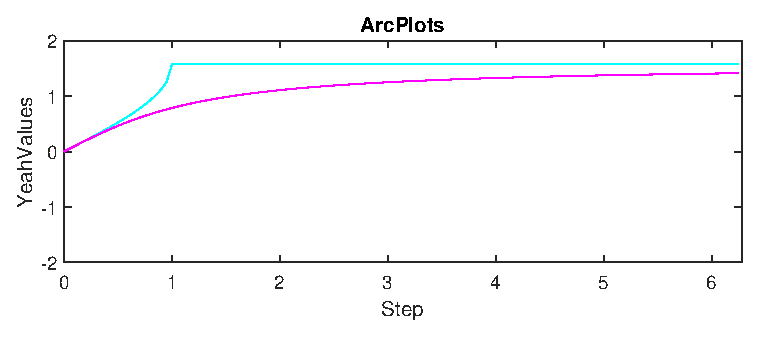
\includegraphics [width=4in]{Exercise_1_01.eps}

\includegraphics [width=4in]{Exercise_1_02.eps}

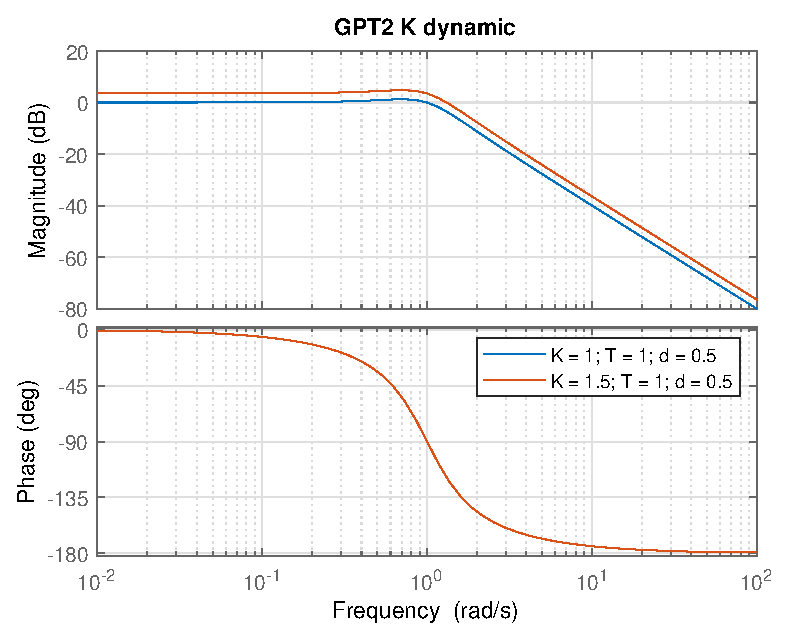
\includegraphics [width=4in]{Exercise_1_03.eps}

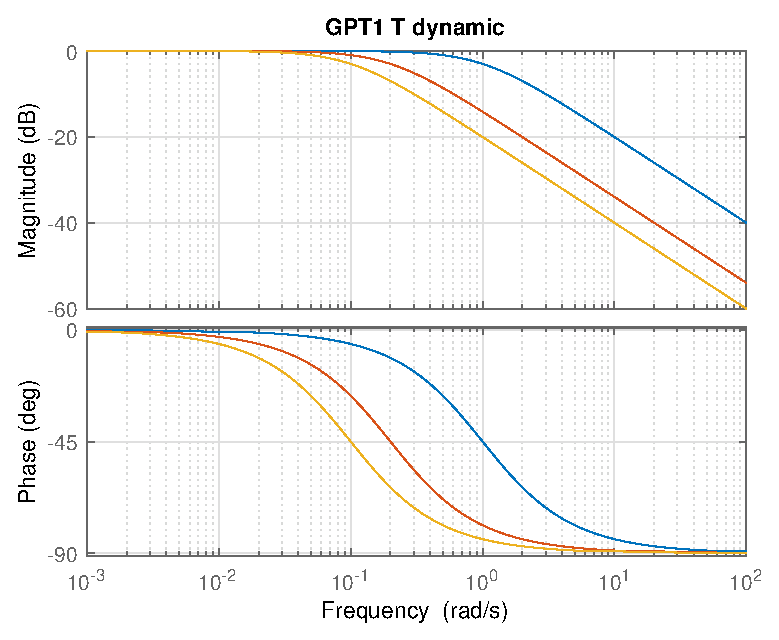
\includegraphics [width=4in]{Exercise_1_04.eps}

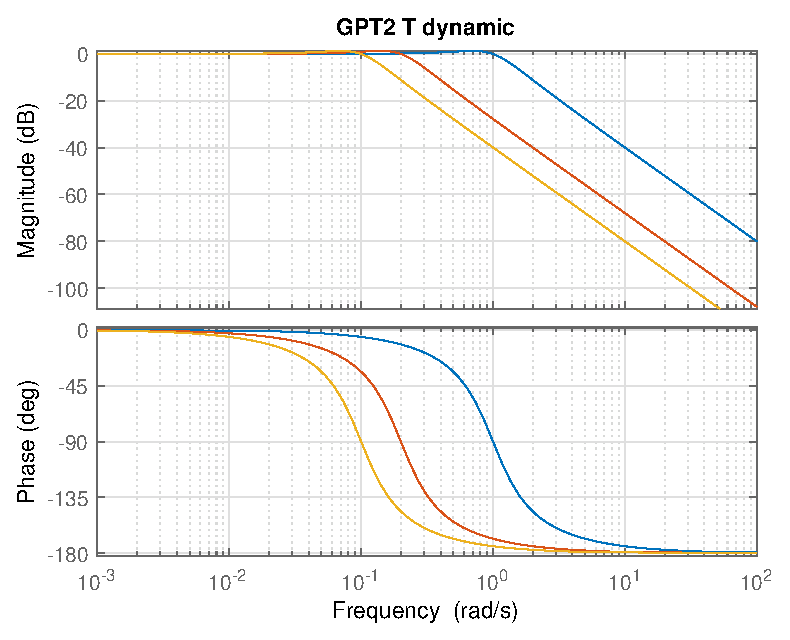
\includegraphics [width=4in]{Exercise_1_05.eps}

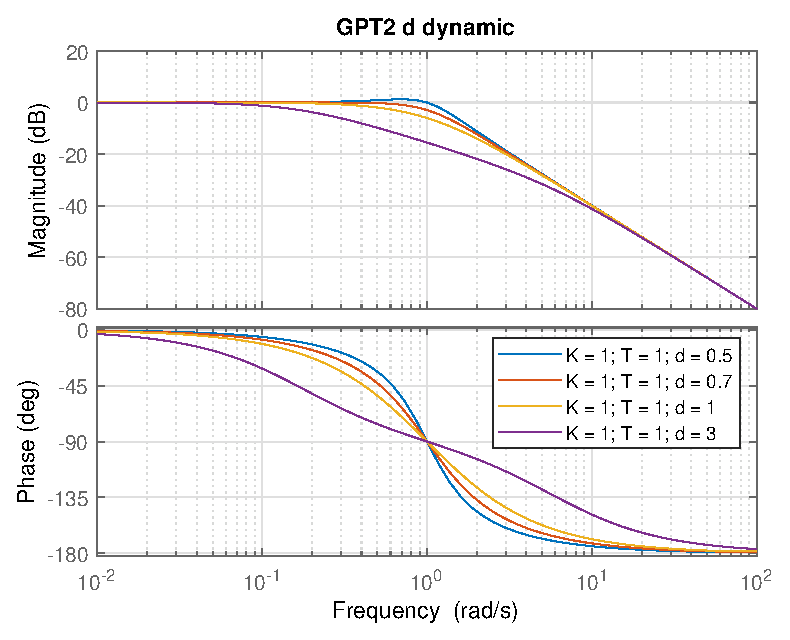
\includegraphics [width=4in]{Exercise_1_06.eps}

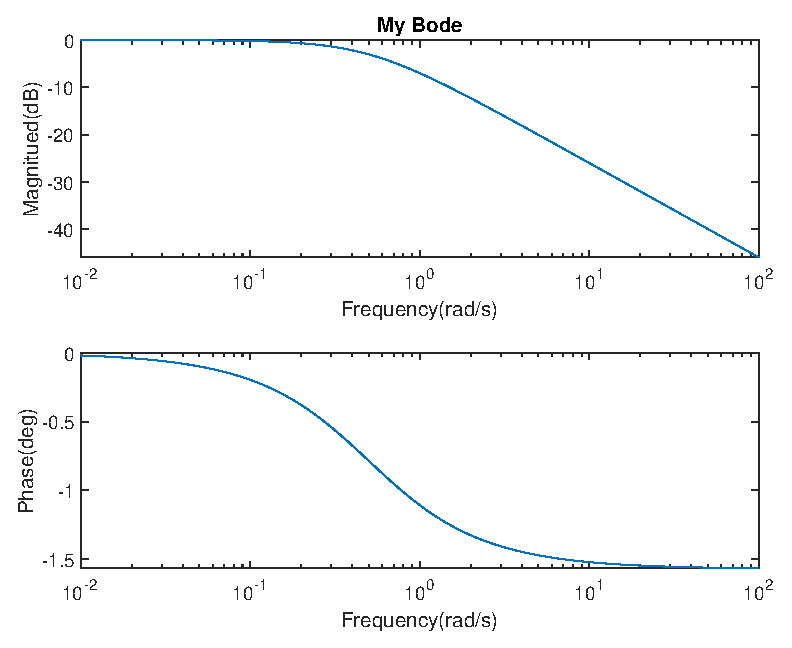
\includegraphics [width=4in]{Exercise_1_07.eps}



\end{document}
    
